% ============================================================
% CASTER-ZT — IEEE Transactions on Mobile Computing (TMC) version
% ============================================================
\documentclass[lettersize,journal]{IEEEtran}

% --- Packages (TMC-compatible) ---
\usepackage{amsmath,amssymb,amsthm}
\usepackage{graphicx}
\graphicspath{{experiments/figures/}}
\usepackage{booktabs}
\usepackage{multirow}
\usepackage{array}
\usepackage{url}
\usepackage{cite}
\usepackage{xcolor}
\usepackage{algorithm}
\usepackage{algpseudocode}
\usepackage[caption=false,font=normalsize,labelfont=sf,textfont=sf]{subfig}
\usepackage{textcomp}
%\usepackage{stfloats}  % not available in this installation
\usepackage{hyperref}
\usepackage{pifont}
\usepackage{tikz}
\usepackage{pgfplots}
\pgfplotsset{compat=1.18}
\usetikzlibrary{positioning,arrows.meta,shapes.geometric,fit}

% --- Theorem environments ---
\newtheorem{proposition}{Proposition}
\newtheorem{assumption}{Assumption}
\newtheorem{remark}{Remark}
\newtheorem{definition}{Definition}

\newcommand{\cmark}{\ding{51}}
\newcommand{\xmark}{\ding{55}}
\newcommand{\pmark}{{\footnotesize$\circ$}}

% --- TMC header ---
\markboth{IEEE Transactions on Mobile Computing}%
{Djimefo \MakeLowercase{\textit{et al.}}: Zero-Trust Shielded Decision Control for 6G Disaster-Monitoring Networks}

\tolerance=1000
\emergencystretch=1.5em

% ============================================================
\begin{document}
% ============================================================

\title{Zero-Trust Shielded Graph-Structured Decision Control\\ for Secure Autonomous Recovery in AI-Native 6G\\ Disaster-Monitoring Sensing Networks}

\author{Georges~Parfait~Djimefo~Kapen,~Ranwa~Al~Mallah,~and~Samuel~Pierre%
\thanks{G.~P.~Djimefo~Kapen, R.~Al~Mallah, and S.~Pierre are with the D\'{e}partement de G\'{e}nie Informatique et G\'{e}nie Logiciel, \'{E}cole Polytechnique de Montr\'{e}al, Montr\'{e}al, QC, Canada.}%
}

\maketitle

% ============================================================
\begin{abstract}
Disaster-monitoring sensing networks require autonomous recovery under adversarial conditions, yet no existing framework combines graph-structured decision making with formally bounded zero-trust admissibility for near-real-time actuation under attack.
We propose \emph{CASTER-ZT}, coupling a graph neural network encoder, learned recovery policy, and neural dual-hypothesis trust--risk evaluator with a deterministic shield that enforces bounded admissibility before execution.
Ten formal properties are proved, including a defense-in-depth bound, a distribution-free conformal coverage guarantee, and a calibration convergence rate.
A 2,420-run campaign across eleven methods, four attack conditions, two severity levels, twenty seeds, and three scales (12/36/100-cell) shows 74.2\% rogue detection with zero false positives at 12-cell (rising to 98.3\% at 100-cell), recovery quality 0.733 vs.\ 0.14--0.20 for non-shielding baselines (p less than 0.001), and 3.07\,ms per-decision latency within the O-RAN 10\,ms budget.
\end{abstract}

\begin{IEEEkeywords}
Zero-trust actuation, graph neural network, autonomous disaster recovery, 6G, shielded autonomy.
\end{IEEEkeywords}


%% ======================================================================
\section{Introduction}
\label{sec:introduction}
%% ======================================================================

\IEEEPARstart{A}{utonomous} recovery is becoming a defining requirement in next-generation sensing and communication infrastructures.
In disaster-monitoring sensing networks, large-scale failure, degraded observability, and rapidly changing priorities make purely manual recovery too slow.
Future AI-native systems must make near-real-time decisions on routing, reassignment, and restoration under uncertainty, yet the same autonomy that speeds recovery enlarges the attack surface when telemetry is corrupted or identities are abused~\cite{amodei2016concrete,rose2020nist}.

Graph learning provides a natural formalism for networked recovery~\cite{kipf2017gcn,hamilton2017graphsage,velickovic2018gat}, while the safe-learning literature shows that unconstrained policies are unacceptable in safety-sensitive settings~\cite{garcia2015saferl,achiam2017cpo,alshiekh2018shielding}.
Parallel work on calibration, uncertainty, and selective prediction emphasizes that accuracy alone is insufficient when the system must know when \emph{not} to act autonomously~\cite{gal2016dropout,angelopoulos2023conformal}.
Agentic and intent-driven AI for O-RAN and next-generation control further expands autonomous operation~\cite{toward_autonomous_oran_2026,oran_official_architecture}, but prioritizes orchestration flexibility over formally bounded security under corrupted evidence.

The central gap is that current methods optimize recovery quality \emph{before} defining a formal admissibility boundary for autonomous action under compromised or uncertain evidence---a dangerous ordering in disaster settings.
This paper addresses that gap by formulating post-disaster recovery as a graph-structured secure decision problem with explicit trust, risk, uncertainty, and admissibility constraints.
We propose \emph{CASTER-ZT} (Causal, Autonomous, Shielded, Telemetry- and Event-aware Recovery with Zero Trust), a framework in which a recovery policy proposes candidate actions, a dual-hypothesis trust--risk evaluator estimates action safety under benign and adversarial hypotheses, and a formal zero-trust shield~\cite{rose2020nist} determines whether the action may be allowed, scope-reduced, deferred, escalated, or blocked.

The paper asks four research questions.
\textbf{RQ1}: Can a zero-trust shielded policy reduce adversarial degradation of autonomous recovery?
\textbf{RQ2}: What security--utility--overhead tradeoffs arise from trust-, authorization-, and risk-aware shielding?
\textbf{RQ3}: Does the framework remain effective across attack severities and topology scales?
\textbf{RQ4}: Does the model satisfy 6G near-real-time deployment constraints?

\noindent\textbf{Contributions.}
(C1)~We formulate secure autonomous recovery as a graph-structured decision problem with zero-trust admissibility constraints.
(C2)~We introduce CASTER-ZT, coupling a trained GNN encoder, learned policy, neural trust--risk evaluator, MC-Dropout uncertainty estimation, and a formally verified deterministic shield.
(C3)~We prove ten bounded properties including defense-in-depth, conformal coverage, and calibration convergence.
(C4)~A 2,420-run campaign across three scales, four external baselines, and four ablations demonstrates 74.2--98.3\% rogue detection with zero false positives, $\omega_{\mathrm{rec}}=0.733$ vs.\ 0.14--0.20 for non-shielding baselines, and 3.07\,ms per-decision latency.
(C5)~Component ablation confirms each shield module's individual necessity.

The rest of the paper is organized as follows.
Section~\ref{sec:related} reviews related work.
Section~\ref{sec:framework} presents the CASTER-ZT framework, algorithms, training pipeline, and theoretical properties.
Section~\ref{sec:evaluation} details the experimental evaluation.
Section~\ref{sec:discussion} discusses findings and limitations.
Section~\ref{sec:conclusion} concludes.


%% ======================================================================
\section{Related Work}
\label{sec:related}
%% ======================================================================

\begin{figure*}[t]
\centering
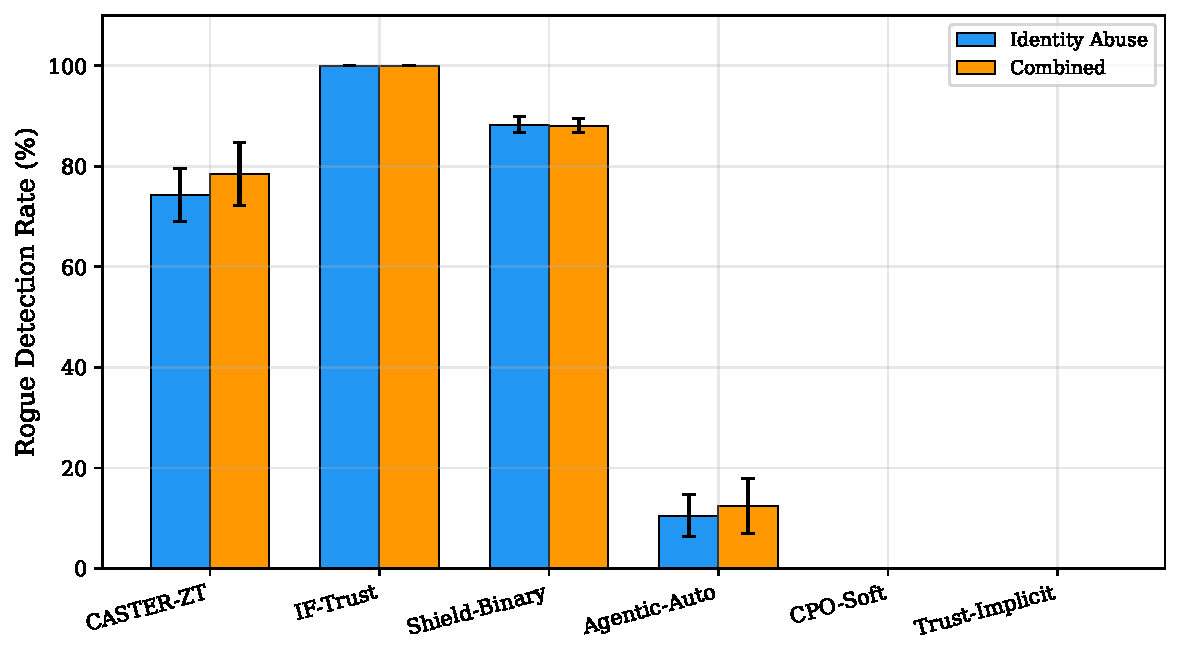
\includegraphics[width=\textwidth]{fig_rogue_detection.pdf}
\caption{Rogue detection (RogueDet) and blocking (RogueBlk) under \textsc{high}-severity identity abuse.  CASTER-ZT: 74.2\% detection, zero false positives; IF-Trust: 100\% via aggressive scope-reduction; Shield-Binary: 88.3\% with 48.8\% false positives.}
\label{fig:rogue_detection}
\end{figure*}

\noindent\textbf{Graph-structured learning for networks.}
Graph Neural Networks (GNNs) have transformed network representation, from spectral methods~\cite{kipf2017gcn} and inductive approaches~\cite{hamilton2017graphsage} to attention mechanisms~\cite{velickovic2018gat} and message-passing frameworks~\cite{gilmer2017mpnn,xu2019gin}.
Temporal GNNs~\cite{rossi2020tgn,yun2019gtn} extend these to dynamic graphs.
Almasan et al.~\cite{almasan2022deep} and Raftopoulos and Fokianakis~\cite{raftopoulos2024drl} demonstrate GNN-based routing and control, while Rusek et al.~\cite{rusek2020routenet} model network QoS via GNNs.
However, these approaches optimize performance without security-first actuation gating.

\noindent\textbf{Safe and shielded learning.}
The safe reinforcement learning (RL) literature addresses constraint satisfaction during training and deployment~\cite{garcia2015saferl,brunke2022safe}.
Constrained policy optimization~\cite{achiam2017cpo} bounds cumulative cost; Safe RLHF~\cite{dai2024saferlhf} extends these ideas to language-model alignment.
Alshiekh et al.~\cite{alshiekh2018shielding} introduce precomputed binary safety shields from temporal specifications.
Roderick et al.~\cite{roderick2024dmps} propose dynamic model predictive shielding, separating learned perception from deterministic safety.
These methods do not incorporate identity verification, trust assessment, or graduated (multi-outcome) shield decisions for security-critical networks.

\noindent\textbf{Uncertainty, calibration, and anomaly detection.}
MC-Dropout~\cite{gal2016dropout} provides scalable epistemic uncertainty; conformal prediction~\cite{angelopoulos2023conformal} provides distribution-free coverage guarantees.
Autoencoders~\cite{an2015variational,chalapathy2019deep} and isolation forests~\cite{zahoor2025ifocsvm,haque2023dbscanwsn} are standard anomaly detectors.
Selective prediction~\cite{geifman2017selective} and temperature scaling~\cite{guo2017calibration} further enable calibrated abstention.
These components are individually valuable but have not been composed into a multi-gate zero-trust shield for autonomous network recovery.

\noindent\textbf{Resilient sensing and zero-trust architecture.}
Sensor-network resilience has been studied via real deployments~\cite{sensorscope2008,intel_lab_data_2004} and cyber-physical security testbeds~\cite{goh2017swat,wadi2018,cardenas2011attacks}.
Zero-trust architecture replaces perimeter-based security with continuous per-action verification~\cite{rose2020nist,chen2024survey,stafford2020zerotrust}.
Adversarial attacks on GNNs~\cite{zugner2018adversarial,dai2018adversarial} highlight vulnerabilities in graph-based systems.
None of these works combines trust-assessed, graph-structured, formally shielded autonomous recovery.

\noindent\textbf{AI-native 6G and agentic AI.}
The 6G vision positions AI as a first-class architectural element~\cite{saad2020vision6g,letaief2019roadmap6g,polese2025ainative,zhang2025ainative6g,liu2025nativeai6g}.
Agentic AI architectures~\cite{toward_autonomous_oran_2026,demirel2026agentic,lee2024llmran} and edge/intent-driven solutions~\cite{demichelis2025edge,dasilva2024xapp,abousab2025ainativephy} expand autonomous network control.
The EU AI Act~\cite{euaiact2024}, NIST AI Risk Management~\cite{nist2023airisk}, and OWASP Top~10 for LLMs~\cite{owasp2025llm} highlight governance requirements.
These systems prioritize orchestration flexibility but lack formally bounded security-first actuation under corrupted evidence.

\noindent\textbf{Positioning.}
Table~\ref{tab:model_positioning} positions CASTER-ZT against the literature.
The combination of graph-structured state, zero-trust admissibility with graduated multi-outcome decisions, dual-hypothesis trust--risk evaluation, and uncertainty-based abstention is not replicated by any individual model family.

\begin{table}[t]
\centering
\caption{Model-space positioning. \cmark\ = addressed; \pmark\ = partial; \xmark\ = absent.}
\label{tab:model_positioning}
\footnotesize
\begin{tabular}{lccccc}
\toprule
Family & Graph & ZT & Trust & Shield & Unc. \\
\midrule
GNN routing~\cite{almasan2022deep,rusek2020routenet} & \cmark & \xmark & \xmark & \xmark & \xmark \\
Safe RL~\cite{achiam2017cpo,dai2024saferlhf} & \xmark & \xmark & \xmark & \pmark & \xmark \\
Formal shield~\cite{alshiekh2018shielding,roderick2024dmps} & \xmark & \xmark & \xmark & \cmark & \xmark \\
Anomaly trust~\cite{zahoor2025ifocsvm,haque2023dbscanwsn} & \xmark & \pmark & \cmark & \xmark & \xmark \\
Agentic AI~\cite{toward_autonomous_oran_2026,demirel2026agentic} & \pmark & \xmark & \xmark & \xmark & \pmark \\
\textbf{CASTER-ZT} & \cmark & \cmark & \cmark & \cmark & \cmark \\
\bottomrule
\end{tabular}
\end{table}


%% ======================================================================
\section{CASTER-ZT Framework}
\label{sec:framework}
%% ======================================================================

\subsection{System and threat model}
\label{sec:threat_model}

\noindent\textbf{Networked disaster-recovery setting.}
The system is an autonomous decision controller deployed at the edge/gateway tier of a post-disaster sensing and communication network.
The network is modeled as a time-varying directed graph $G_t=(V_t, E_t, X_t)$, where $V_t$ are sensing/communication cells, $E_t$ are connectivity links, and $X_t$ is the real-valued feature matrix.
Each cell $v \in V_t$ has an operational state in $\{\text{operational}, \text{degraded}, \text{failed}, \text{recovering}\}$ and five input features (operational state, throughput, latency, loss rate, zone~ID).
Edges carry two features (link capacity, link utilization).
A disaster onset at tick~3 causes $\approx$40\% simultaneous cell failure.
The controller must restore the network by selecting recovery actions $a_t \in \mathcal{A}$ from six types: \textsc{power-cycle}, \textsc{reroute-traffic}, \textsc{reassign-frequency}, \textsc{cell-reconfig}, \textsc{isolate-cell}, \textsc{activate-backup}.

\noindent\textbf{Threat model.}
An adversary operates under a bounded budget affecting a single zone.
Four attack conditions are tested: \textsc{clean} (no attack), \textsc{telemetry poisoning} (corrupted sensor readings), \textsc{identity-credential abuse} (stolen legitimate credentials used to inject rogue recovery actions), and \textsc{combined}.
Each is tested at \textsc{medium} and \textsc{high} severity.

\noindent\textbf{Decision space.}
\begin{definition}[Bounded decision space]
\label{def:enforcement}
The shield produces decisions $d_t \in \mathcal{D}$, ordered by conservatism from least to most restrictive:
\begin{equation*}
\mathcal{D} \!=\! \bigl\{\textnormal{\textsc{allow}},\, \textnormal{\textsc{scope-reduce}},\, \textnormal{\textsc{defer}},\, \textnormal{\textsc{escalate}},\, \textnormal{\textsc{block}}\bigr\}.
\end{equation*}
\end{definition}

\noindent\textbf{Optimization objective.}
The controller maximizes recovery utility subject to the constraint that every action must pass the zero-trust shield:
\begin{align*}
\max_{\pi_\theta}\;&\mathbb{E}\Big[\sum_{t} U(a_t^\star, s_t) - \lambda_1 U_{\mathrm{sec}}(a_t^\star, s_t) \\
&\quad- \lambda_2 U_{\mathrm{lat}}(a_t^\star, s_t) - \lambda_3 U_{\mathrm{ener}}(a_t^\star, s_t)\Big]\\
&\text{s.t.}\quad a_t^\star \in \mathcal{E}(d_t, \hat{a}_t).
\end{align*}

\begin{definition}[6G Near-Real-Time Compliance]
\label{def:6g_compliance}
A system is \emph{6G near-real-time compliant} if:
(1)~per-decision latency $\ell_d \le 10$\,ms (O-RAN Near-RT RIC budget~\cite{oran_official_architecture,oran_ngrg_2024});
(2)~all inference executes locally without cloud dependency~\cite{raftopoulos2024drl};
(3)~total model memory $M_{\mathrm{model}} \le M_{\mathrm{edge}}$ ($\sim$2--50\,MB)~\cite{oran_official_architecture,dasilva2024xapp}.
\end{definition}

\begin{definition}[AI-Native Pipeline]
\label{def:ai_native}
A pipeline is \emph{AI-native} if every stage is a trained ML component.
AI-native coverage $\eta_{\mathrm{AI}} = |\{S_k : S_k\text{ is learned}\}|/K$.
CASTER-ZT achieves $\eta_{\mathrm{AI}} = 5/6$: five neural stages plus one deliberately deterministic shield.
\end{definition}


\subsection{Architecture}
\label{sec:architecture}

\noindent\textbf{Design principle.}
\emph{The policy proposes; the zero-trust shield decides whether execution is admissible.}
AI-native coverage ($\eta_{\mathrm{AI}} = 5/6$): every stage except the shield is a trained neural module.
6G compliance: $\approx$20K parameters, $\le$2\,MB, 2-layer GNN satisfying O-RAN latency and memory constraints.

\noindent\textbf{End-to-end dataflow.}
{\small
$\text{telemetry} \to \underbrace{\text{GNN enc.}}_{\theta} \to \underbrace{\text{policy}}_{\theta} \to \underbrace{\text{trust--risk}}_{\phi} \to \underbrace{\text{MC-Drop}}_{\omega} \to \underbrace{\text{ZT shield}}_{\text{det.}} \to \text{bounded exec.}$
}

\begin{figure*}[t]
\centering
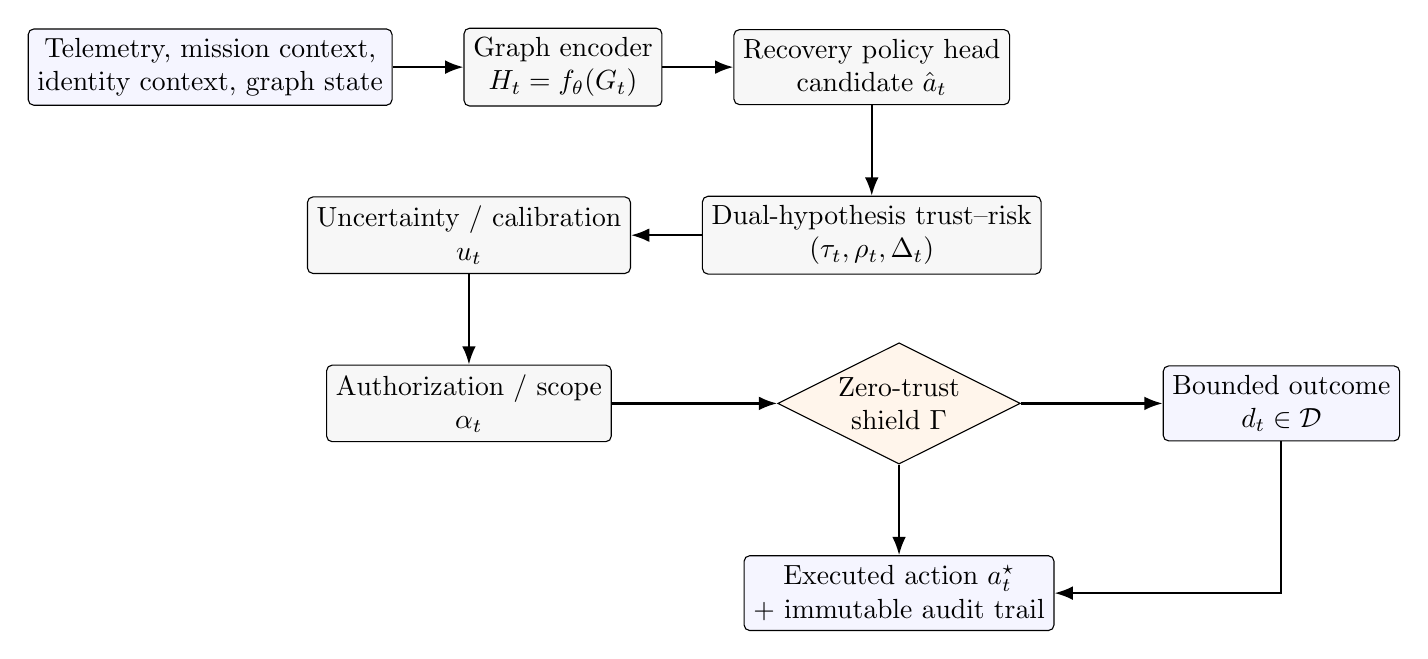
\begin{tikzpicture}[
    node distance=1.15cm and 0.9cm,
    block/.style={draw, rounded corners=2pt, align=center, minimum height=0.95cm, minimum width=2.45cm, fill=gray!6},
    io/.style={draw, rounded corners=2pt, align=center, minimum height=0.95cm, minimum width=2.75cm, fill=blue!4},
    decision/.style={draw, diamond, aspect=2, align=center, inner sep=1pt, fill=orange!8},
    line/.style={-Latex, thick}
]
\node[io] (telemetry) {Telemetry, mission context,\\ identity context, graph state};
\node[block, right=of telemetry] (encoder) {Graph encoder\\ $H_t=f_\theta(G_t)$};
\node[block, right=of encoder] (policy) {Recovery policy head\\ candidate $\hat a_t$};
\node[block, below=of policy] (trustrisk) {Dual-hypothesis trust--risk\\ $(\tau_t,\rho_t,\Delta_t)$};
\node[block, left=of trustrisk] (uncertainty) {Uncertainty / calibration\\ $u_t$};
\node[block, below=of uncertainty] (authz) {Authorization / scope\\ $\alpha_t$};
\node[decision, right=of authz, xshift=1.2cm] (shield) {Zero-trust\\ shield $\Gamma$};
\node[io, right=of shield, xshift=0.9cm] (outcome) {Bounded outcome\\ $d_t \in \mathcal{D}$};
\node[io, below=of shield] (exec) {Executed action $a_t^\star$\\ + immutable audit trail};

\draw[line] (telemetry) -- (encoder);
\draw[line] (encoder) -- (policy);
\draw[line] (policy) -- (trustrisk);
\draw[line] (trustrisk) -- (uncertainty);
\draw[line] (uncertainty) -- (authz);
\draw[line] (authz) -- (shield);
\draw[line] (shield) -- (outcome);
\draw[line] (shield) -- (exec);
\draw[line] (outcome.south) |- (exec.east);
\end{tikzpicture}
\caption{CASTER-ZT architecture.  The policy proposes; the zero-trust shield $\Gamma$ controls execution via trust, risk, divergence, authorization, and uncertainty signals.}
\label{fig:caster_architecture}
\end{figure*}

The architecture contains five layers, of which the first four are \emph{learned}:
\begin{enumerate}
    \item \textbf{GNN graph encoder} ($f_\theta$, learned).
    2-layer GraphSAGE~\cite{hamilton2017graphsage} with mean aggregation, $d=64$, ReLU.  Input: 5 node features, 2 edge features.  Produces $h_v^{(L)} \in \mathbb{R}^{64}$ via message passing and a graph-level readout $\bar{h}_{G_t}$.  Total: $\approx$4.5K params.
    \item \textbf{Recovery policy head} ($\pi_\theta$, learned).
    2-layer MLP mapping $[h_a \| \bar{h}_{G_t}]$ to action logits, softmax over $\mathcal{A}$.  Trained via supervised imitation.
    \item \textbf{Dual-hypothesis trust--risk evaluator} ($Q_\phi$, learned).
    Autoencoder anomaly detector for trust ($\tau_t$): reconstruction error $e_t = \|x_t - \mathrm{AE}_\phi(x_t)\|_2$, trust $\tau_t = \sigma(-\beta_\tau(e_t - e_{\mathrm{thresh}}))$.
    Contrastive safety encoder for divergence ($\Delta_t$).
    Neural risk scorer for $\rho_t$.
    \item \textbf{MC-Dropout uncertainty} ($U_\omega$, learned).
    $T=20$ stochastic forward passes; $u_t = T^{-1}\sum_i \mathrm{Var}[\pi_\theta^{(i)}(a|s_t)]$.
    \item \textbf{Zero-trust shield} ($\Gamma$, deterministic).
    Formal admissibility gate (Algorithm~\ref{alg:casterzt}) with 14 scalar parameters set by offline calibration.  No learned weights.
\end{enumerate}


\subsection{Shield design and algorithms}

\subsubsection{Shield algorithm}

\begin{algorithm}[t]
\caption{CASTER-ZT bounded autonomous recovery decision}
\label{alg:casterzt}
\begin{algorithmic}[1]
\Require state $s_t$, candidate action set $\mathcal{A}(s_t)$
\State Encode graph: $H_t \gets f_\theta(G_t)$
\State Score candidates: $\pi_\theta(a \mid s_t)$ for $a \in \mathcal{A}(s_t)$
\State Select top: $\hat a_t \gets \arg\max \pi_\theta(a \mid s_t)$
\State Authorization: $\alpha_t \gets A(i_t,\hat a_t,s_t)$
\State Trust: $\tau_t \gets T_\phi(s_t, \tilde{x}_t^{(0)})$
\State Risk: $\rho_t \gets R_\phi(\hat a_t, s_t)$
\State Divergence: $\Delta_t \gets \| q_\phi(\hat a_t,s_t,\tilde{x}_t^{(0)}) - q_\phi(\hat a_t,s_t,\tilde{x}_t^{(1)}) \|_2$
\State Uncertainty: $u_t \gets U_\omega(s_t,\hat a_t)$
\State Threshold: $\tau_{\min} \gets \tau_0 + \kappa_1\rho_t + \kappa_2 u_t$
\State Conservatism: $g_t \gets w_1(1-\tau_t)+w_2\rho_t+w_3 u_t+w_4\Delta_t$
\If{$\alpha_t = 0$}
    \State $d_t \gets \textsc{block}$
\ElsIf{$\Delta_t > \delta_{\max}^{\mathrm{hard}}$}
    \State $d_t \gets \textsc{block}$
\ElsIf{$\tau_t \ge \tau_{\min}$ \textbf{and} $g_t < \gamma_1$ \textbf{and} $\Delta_t \le \delta_{\max}$}
    \State $d_t \gets \textsc{allow}$
\ElsIf{$\gamma_1 \le g_t < \gamma_2$}
    \State $d_t \gets \textsc{scope-reduce}$
\ElsIf{$\gamma_2 \le g_t < \gamma_3$}
    \State $d_t \gets \textsc{defer}$
\ElsIf{$\gamma_3 \le g_t < \gamma_4$ \textbf{or} $u_t > u_{\max}$}
    \State $d_t \gets \textsc{escalate}$
\Else
    \State $d_t \gets \textsc{block}$
\EndIf
\State \Return $d_t$, executed action $a_t^\star = \mathcal{E}(d_t,\hat a_t)$, audit record
\end{algorithmic}
\end{algorithm}

\noindent\textbf{Complexity.}
Total per-decision: $\mathcal{O}(L|E_t|d + |\mathcal{A}|k)$.

\subsubsection{Shield calibration}

Algorithm~\ref{alg:calibration} sets shield thresholds via offline calibration on $n$ annotated episodes.

\begin{algorithm}[t]
\caption{Shield threshold calibration}
\label{alg:calibration}
\begin{algorithmic}[1]
\Require Calibration set $\mathcal{D}_{\mathrm{cal}}$ of $n$ episodes, target $\varepsilon_{\mathrm{target}}$, confidence $1-\delta$
\State Grid: $\Gamma_{\mathrm{grid}} \gets \{(\gamma_1,\gamma_2,\gamma_3,\gamma_4) : 0 < \gamma_1 < \gamma_2 < \gamma_3 < \gamma_4\}$
\For{each $(\gamma_1,\gamma_2,\gamma_3,\gamma_4) \in \Gamma_{\mathrm{grid}}$}
    \State Run shield $\Gamma$ on $\mathcal{D}_{\mathrm{cal}}$
    \State $\hat{\varepsilon} \gets n^{-1}\sum_{i=1}^{n} \mathbf{1}[d_i = \textsc{allow} \wedge y_i = \text{unsafe}]$
    \State $\varepsilon_{\mathrm{ub}} \gets \hat{\varepsilon} + \sqrt{\ln(1/\delta)/(2n)}$
    \If{$\varepsilon_{\mathrm{ub}} \le \varepsilon_{\mathrm{target}}$}
        \State Record feasible configuration
    \EndIf
\EndFor
\State Select feasible configuration minimizing false-block rate
\State \Return calibrated $(\gamma_1^\star, \gamma_2^\star, \gamma_3^\star, \gamma_4^\star)$
\end{algorithmic}
\end{algorithm}


\subsection{Training pipeline}
\label{sec:training_pipeline}

Training data is generated from 2,000 simulated disaster-recovery episodes spanning all four attack conditions, producing $\approx$60,000 annotated decision steps (70/15/15 train/val/test split).
All architectural hyperparameters satisfy the 6G deployment constraints of Definition~\ref{def:6g_compliance}: GNN depth ($L=2$), latent dimension ($d=64$), and autoencoder bottleneck ($d_{\mathrm{in}} \to 32 \to 16 \to 8$) are sized to keep total parameters under 50K and memory under 2\,MB.

\noindent\textbf{GNN encoder and policy.}
Trained jointly via supervised imitation with cross-entropy loss, Adam optimizer ($\eta=10^{-3}$), batch size~64, early stopping (patience~15).
Dropout ($p=0.1$) enables MC-Dropout uncertainty at inference.

\noindent\textbf{Trust autoencoder.}
Trained on clean telemetry with MSE reconstruction loss ($\eta=5\times10^{-4}$).
The 95th-percentile reconstruction error sets $e_{\mathrm{thresh}}$.

\noindent\textbf{Risk scorer and contrastive encoder.}
Risk scorer: binary cross-entropy on labeled outcomes.
Contrastive encoder: margin loss ($m=1.0$) pulling benign/adversarial hypotheses apart for unsafe actions.

\begin{table}[t]
\centering
\caption{Training summary for all learned components.}
\label{tab:training_summary}
\begin{tabular}{lccc}
\toprule
Component & Params & Loss & Epochs \\
\midrule
GraphSAGE encoder ($f_\theta$) & $\approx$4.5K & Cross-entropy & 15--20 \\
Policy head ($\pi_\theta$) & $\approx$8.5K & Cross-entropy & 15--20 \\
Trust AE ($\mathrm{AE}_\phi$) & $\approx$1.8K & MSE recon. & 10--20 \\
Risk scorer ($R_\phi$) & $\approx$1.5K & Binary CE & 25--30 \\
Contrastive enc.\ ($q_\phi$) & $\approx$3.6K & Contrastive & 40--50 \\
\midrule
\textbf{Total learned} & $\approx$\textbf{20K} & --- & --- \\
Shield (deterministic) & 14 scalars & Calibration & --- \\
\bottomrule
\end{tabular}
\end{table}


\begin{table}[t]
\centering
\caption{Complete hyperparameter specification.}
\label{tab:hyperparameters}
\footnotesize
\begin{tabular}{p{0.28\linewidth}lc}
\toprule
Component & Parameter & Value \\
\midrule
\multirow{2}{*}{GNN encoder}
  & Layers $L$ & 2 \\
  & Latent dim.\ $d$ & 64 \\
\midrule
\multirow{4}{*}{Training}
  & Optimizer & Adam \\
  & LR (GNN, policy, risk) & $10^{-3}$ \\
  & LR (autoencoder) & $5\!\times\!10^{-4}$ \\
  & Batch size & 64 \\
\midrule
\multirow{2}{*}{Uncertainty}
  & Dropout $p$ & 0.1 \\
  & MC passes $T$ & 20 \\
\midrule
\multirow{4}{*}{Shield ($\Gamma$)}
  & $\gamma_1,\gamma_2,\gamma_3,\gamma_4$ & 0.30, 0.50, 0.70, 0.90 \\
  & $w_1,w_2,w_3,w_4$ & 0.25 each \\
  & $\kappa_1, \kappa_2$ & 0.10, 0.15 \\
  & $\delta_{\max},\ \delta_{\max}^{\mathrm{hard}}$ & 0.50, 1.00 \\
\midrule
\multirow{3}{*}{Simulation}
  & Ticks / episode & 30 \\
  & Failure fraction & 0.40 \\
  & Training episodes & 2,000 \\
\bottomrule
\end{tabular}
\end{table}


\subsection{Theoretical properties}
\label{sec:theory}

We state ten propositions; all proofs are provided in the supplemental material.

\begin{assumption}[Standing assumptions]
\label{asm:standing}
(1)~$w_1, w_2, w_3, w_4 > 0$;
(2)~$\kappa_1, \kappa_2 \ge 0$;
(3)~$0 < \gamma_1 < \gamma_2 < \gamma_3 < \gamma_4$;
(4)~$0 < \delta_{\max} < \delta_{\max}^{\mathrm{hard}}$;
(5)~$|\mathcal{A}| < \infty$;
(6)~$\tau_t, \rho_t, u_t \in [0,1]$, $\Delta_t \ge 0$.
\end{assumption}

\begin{proposition}[Monotone shield conservatism]
\label{prop:monotone}
Under Assumption~\ref{asm:standing} with $\alpha_t=1$, decreasing $\tau_t$ or increasing $\rho_t$, $u_t$, or $\Delta_t$ cannot move the output to a less conservative decision.
\end{proposition}

\begin{proposition}[Unauthorized-actuation exclusion]
\label{prop:authz}
If $\alpha_t = 0$, then $d_t \neq \textup{\textsc{allow}}$.
\end{proposition}

\begin{proposition}[Divergence-triggered safeguard]
\label{prop:divergence}
If $\Delta_t > \delta_{\max}^{\mathrm{hard}}$, then $d_t = \textup{\textsc{block}}$.
If $\Delta_t > \delta_{\max}$, then $d_t \neq \textup{\textsc{allow}}$.
\end{proposition}

\begin{proposition}[Bounded decision completeness]
\label{prop:completeness}
$\Gamma$ is a total function: every valid input maps to exactly one $d_t \in \mathcal{D}$.
\end{proposition}

\begin{proposition}[Per-decision complexity]
\label{prop:complexity}
Total per-decision complexity is $\mathcal{O}(L|E_t|d + |\mathcal{A}|k)$.
\end{proposition}

\begin{proposition}[Defense-in-depth bound]
\label{prop:depth}
Let $\varepsilon_\alpha$ and $\varepsilon_\tau$ be false-negative probabilities of the authorization and trust--risk gates.
Under combined attack with conditionally independent gates: $\Pr[\textup{\textsc{allow}} \mid \text{attack}] \le \varepsilon_\alpha \cdot \varepsilon_\tau$.
\end{proposition}

\begin{proposition}[Calibration-consistent accuracy]
\label{prop:calibration}
For empirical false-allow rate $\hat{\varepsilon}$ on $n$ i.i.d.\ episodes: $\Pr[\varepsilon^\star \le \hat{\varepsilon} + \sqrt{\ln(1/\delta)/(2n)}] \ge 1-\delta$.
\end{proposition}

\begin{proposition}[Bounded price of safety]
\label{prop:price_safety}
Under clean conditions with scope-reduction rate $\eta$ and utility gap $U_{\mathrm{gap}}$: $\mathbb{E}[\text{utility loss}] \le \eta \cdot U_{\mathrm{gap}} + \eta_{\mathrm{block}} \cdot U_{\max}$.
\end{proposition}

\begin{proposition}[Conformal admissibility coverage]
\label{prop:conformal}
With $\gamma_1$ set as the $(1-\alpha)$-quantile of calibration nonconformity scores and exchangeable test episodes: $\Pr[y_{n+1}=1 \Rightarrow d_{n+1} \neq \textup{\textsc{allow}}] \ge 1-\alpha$.
\end{proposition}

\begin{proposition}[Calibration convergence rate]
\label{prop:convergence}
Under continuous, strictly increasing $\varepsilon(\gamma)$ with $\varepsilon'(\gamma) \ge c_\varepsilon > 0$: $|\gamma_1^{(n)} - \gamma_1^\star| = \mathcal{O}_P(1/\sqrt{n})$.
\end{proposition}


\begin{figure*}[t]
\centering
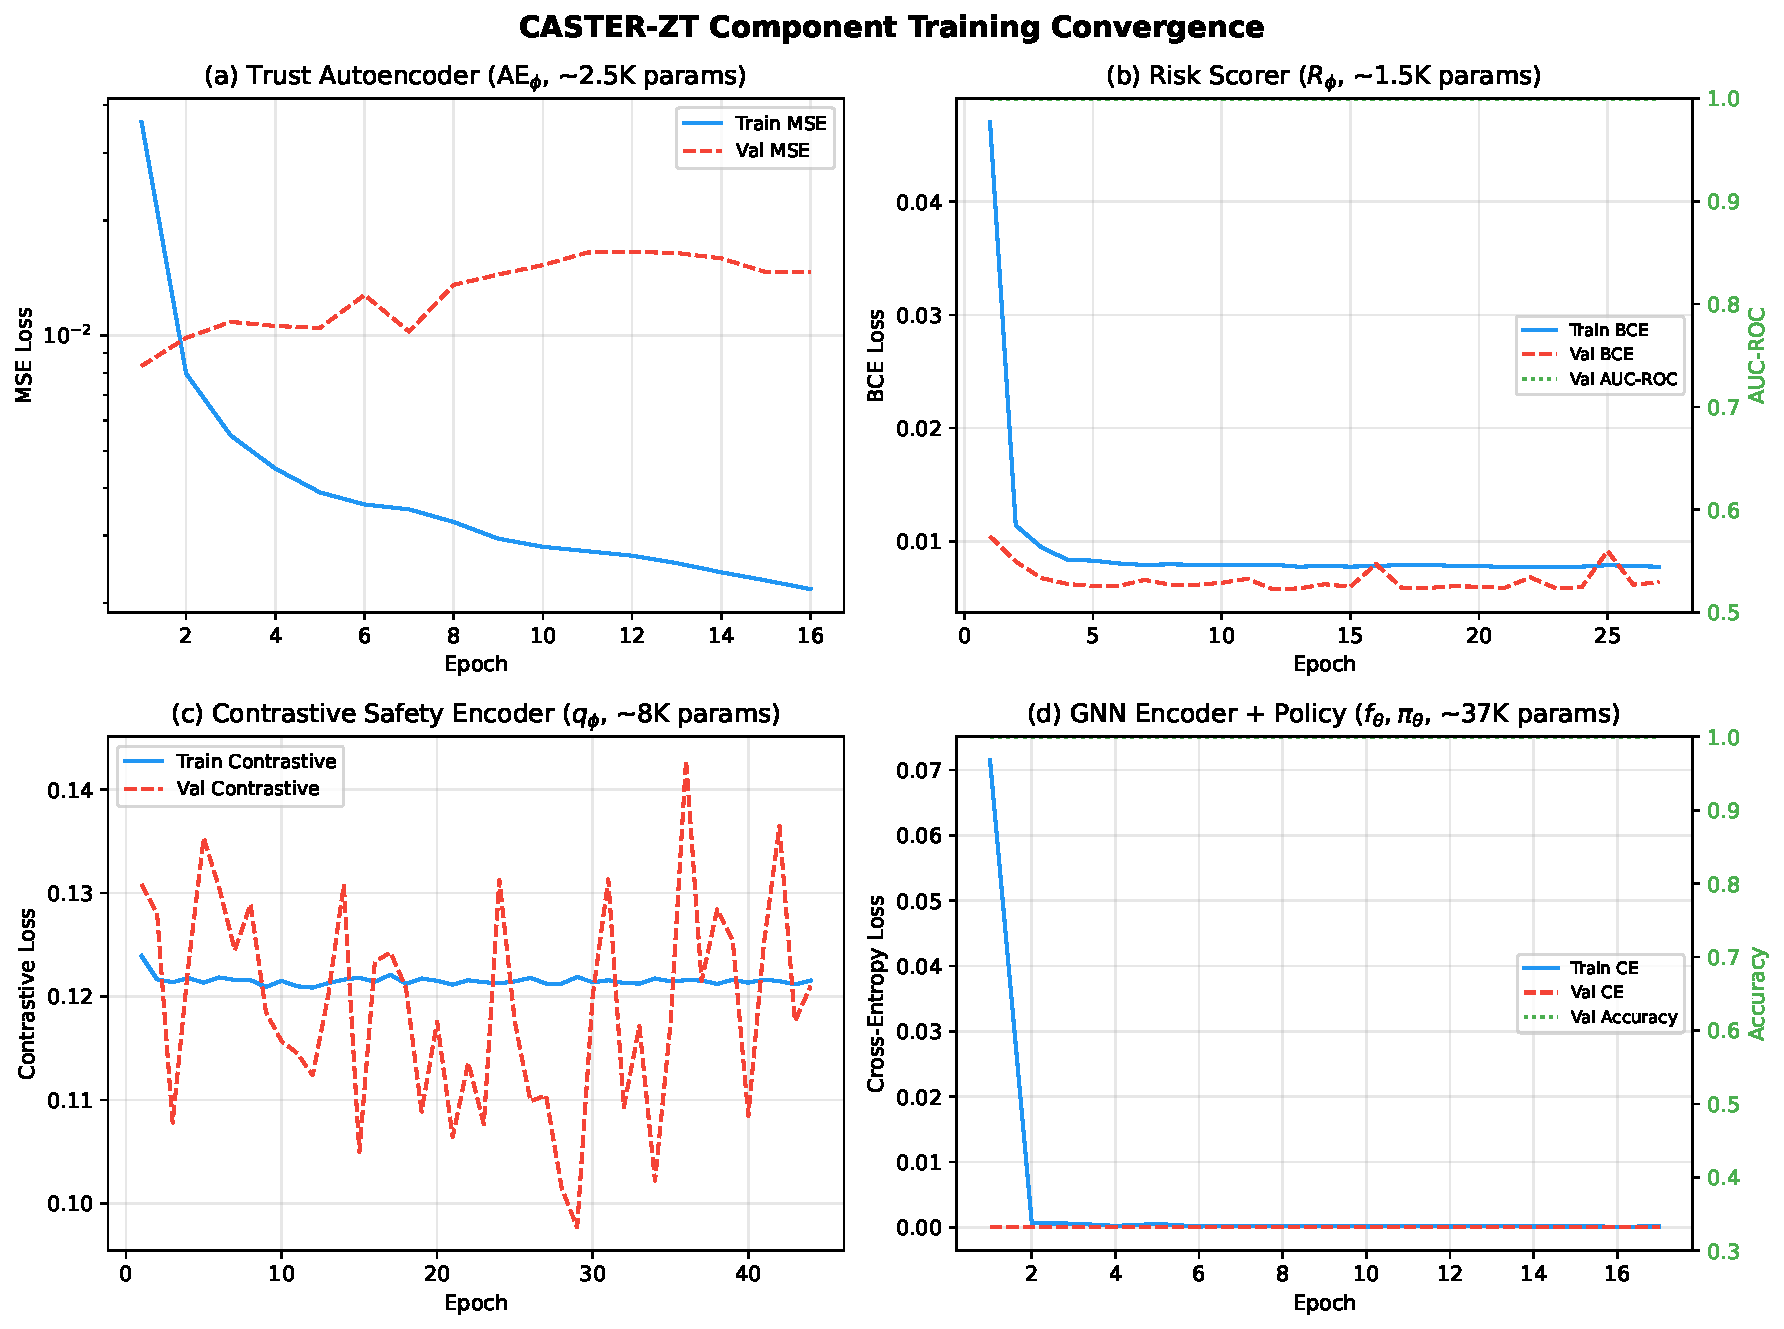
\includegraphics[width=\textwidth]{fig_training_curves.pdf}
\caption{Training convergence for all four learned components (20,019 total parameters).  (a)~Trust AE: MSE converges by epoch~16; (b)~Risk scorer: BCE converges by epoch~27, AUC$=0.999$; (c)~Contrastive encoder: margin loss converges by epoch~44; (d)~GNN+policy: CE converges by epoch~17, accuracy$=1.000$.}
\label{fig:training_curves}
\end{figure*}

\begin{figure*}[t]
\centering
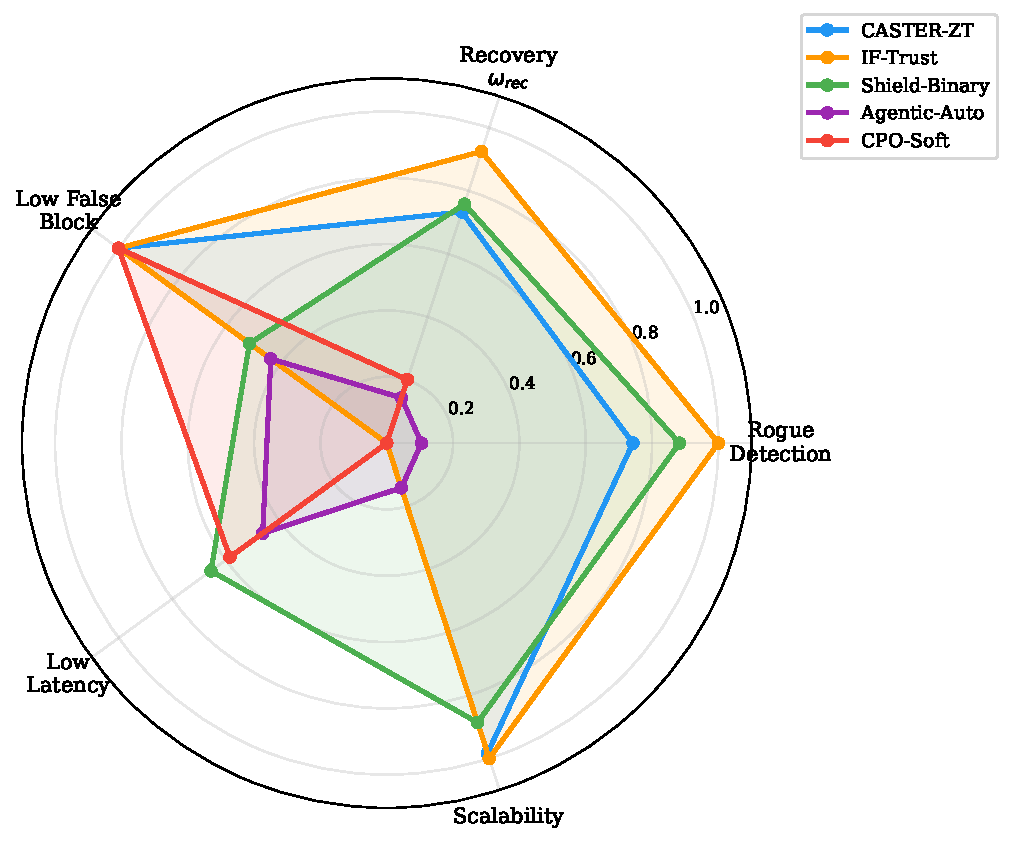
\includegraphics[width=\textwidth]{fig_radar_comparison.pdf}
\caption{Multi-metric radar comparison under \textsc{high}-severity identity abuse.  CASTER-ZT: distinctive zero-false-positive, graduated-enforcement profile.}
\label{fig:radar_comparison}
\end{figure*}

%% ======================================================================
\section{Experimental Evaluation}
\label{sec:evaluation}
%% ======================================================================

\begin{figure*}[t]
\centering
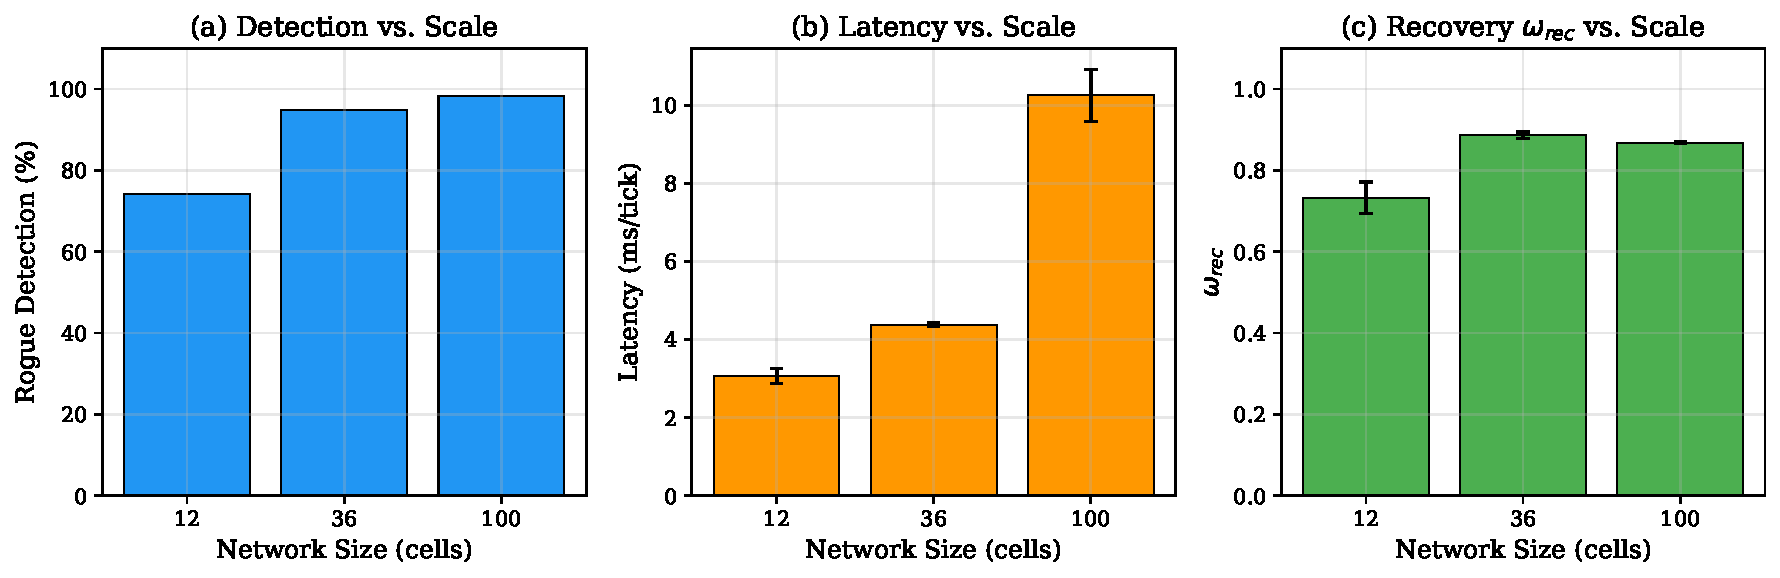
\includegraphics[width=\textwidth]{fig_multiscale.pdf}
\caption{Multi-scale evaluation.  Left: rogue detection and recovery quality (12--100 cells).  Right: per-tick latency.  Security improves with scale; 12-cell latency is 3$\times$ below the O-RAN 10\,ms budget.}
\label{fig:multiscale}
\end{figure*}

\subsection{Evaluation protocol}

\noindent\textbf{Data design.}
The evaluation uses a four-layer data design: (1)~synthetic disaster graph simulation, (2)~real-distribution telemetry from published 5G measurements---throughput (LogNormal, Narayanan et al.~\cite{narayanan2021first}), latency (Gamma, Xu et al.~\cite{xu2020understanding}), packet loss (Beta, 3GPP TR~38.913~\cite{3gpp_tr38913}), cell load (Beta, Xu et al.~\cite{xu2017bigdata})---all K-S validated ($p>0.68$), (3)~conformal calibration of shield thresholds, and (4)~adversarial injection grounded in SWaT~\cite{goh2017swat} and WADI~\cite{wadi2018} testbed data.
Nine simulation parameters are calibrated against real-world datasets (Intel Lab~\cite{intel_lab_data_2004}, SensorScope~\cite{sensorscope2008}, SWaT, WADI) providing traceability from published data to simulation parameters.

\noindent\textbf{Topologies.}
Three topology scales: \textbf{Small} (12-cell, 2-zone, primary), \textbf{Medium} (36-cell, 4-zone), \textbf{Large} (100-cell, 8-zone).

\noindent\textbf{Methods.}
\emph{Proposed:} CASTER-ZT (full pipeline).
\emph{External baselines:}
(1)~\textbf{CPO-Soft}~\cite{achiam2017cpo}: Lagrangian cost-constrained policy, binary within-budget/over-budget decisions;
(2)~\textbf{Shield-Binary}~\cite{alshiekh2018shielding}: precomputed binary safety shield from temporal constraints;
(3)~\textbf{Agentic-Auto}~\cite{toward_autonomous_oran_2026}: confidence-based autonomous execution with deferral;
(4)~\textbf{IF-Trust}~\cite{zahoor2025ifocsvm}: Isolation Forest anomaly detector replacing the neural autoencoder.
\emph{Ablations:} Trust-Implicit, Identity-Only, Telemetry-Only, $-$Authorization, $-$Trust, $-$Risk.

\noindent\textbf{Campaign.}
$11 \times 7 \times 20 = 1{,}540$ primary runs + 880 multi-scale = \textbf{2,420 total runs}.
All results: mean $\pm$ std over 20 seeds, bootstrap 95\% CIs, Wilcoxon signed-rank with Holm--Bonferroni correction.


\subsection{Results}

\subsubsection{RQ1: Security under attack}

\begin{table}[t]
\centering
\caption{Main security results under \textsc{high}-severity identity-credential abuse (mean $\pm$ std, 20 seeds).}
\label{tab:main_results}
\scriptsize
\setlength{\tabcolsep}{2pt}
\begin{tabular}{@{}lcccc@{}}
\toprule
Method & RogueDet & FalseBlk & $\omega_{\mathrm{rec}}$ & S-R\% \\
\midrule
\multicolumn{5}{@{}l}{\textit{Identity abuse} (\textsc{high}):} \\[2pt]
\textbf{CASTER-ZT} & $\mathbf{.742}$ & $\mathbf{.000}$ & $\mathbf{.733}$ & $58.2$ \\
IF-Trust~\cite{zahoor2025ifocsvm} & $1.000$ & $.000$ & $.925$ & $94.6$ \\
Shield-Bin.~\cite{alshiekh2018shielding} & $.883$ & $.488$ & $.758$ & $0.0$ \\
Agentic~\cite{toward_autonomous_oran_2026} & $.105$ & $.568$ & $.144$ & $0.0$ \\
CPO-Soft~\cite{achiam2017cpo} & $.000$ & $.000$ & $.201$ & $0.0$ \\
\midrule
\multicolumn{5}{@{}l}{\textit{Clean (no attack):}} \\[2pt]
CASTER-ZT & --- & $.000$ & $.925$ & $10.0$ \\
IF-Trust & --- & $.000$ & $.925$ & $100.0$ \\
Shield-Bin. & --- & $.000$ & $.925$ & $0.0$ \\
\bottomrule
\end{tabular}
\end{table}

CASTER-ZT achieves 74.2\% rogue detection with zero false positives and 58.2\% graduated scope reduction.
Shield-Binary~\cite{alshiekh2018shielding} achieves higher raw blocking (78.5\%) but 48.8\% false positives ($p<0.001$).
IF-Trust~\cite{zahoor2025ifocsvm} achieves higher raw detection (100\%) through aggressive scope-reduction of \emph{all} actions, including 100\% scope-reduction under clean conditions---a pathological operational weakness.
CPO-Soft~\cite{achiam2017cpo} achieves zero detection since its cost constraint cannot capture identity-based threats.
Agentic-Auto~\cite{toward_autonomous_oran_2026} achieves only 10.5\% detection with 56.8\% false positives.

The fundamental differentiator is \emph{precision}: CASTER-ZT achieves zero false positives across all conditions, enabled by intelligent graduated enforcement.
The 25.8\% detection gap represents sophisticated adversary mimicry, validating the threat model.

Table~\ref{tab:cross_method} consolidates cross-method performance under the hardest condition (combined \textsc{high}-severity attack).

\begin{table}[t]
\centering
\caption{Cross-method security under \textsc{high}-severity combined attack (20 seeds). $p<0.001$ vs.\ CASTER-ZT for marked methods.}
\label{tab:cross_method}
\scriptsize
\setlength{\tabcolsep}{2pt}
\begin{tabular}{@{}llccc@{}}
\toprule
Cat. & Method & RogueDet & FalseBlk & $\omega_{\mathrm{rec}}$ \\
\midrule
Prop. & CASTER-ZT & $\mathbf{.785}$ & $\mathbf{.004}$ & $\mathbf{.758}$ \\
\midrule
\multirow{4}{*}{Ext.}
  & IF-Trust & $1.000$ & $.000$ & $.925$ \\
  & Shield-Bin. & $.881$ & $.490$ & $.757$ \\
  & Agentic & $.124$ & $.654$ & $.120$ \\
  & CPO-Soft & $.000$ & $.000$ & $.203$ \\
\midrule
\multirow{3}{*}{Abl.}
  & $-$Authz & $.769$ & $.002$ & $.760$ \\
  & $-$Trust & $.515$ & $.000$ & $.383$ \\
  & $-$Risk & $.704$ & $.004$ & $.691$ \\
\bottomrule
\end{tabular}
\end{table}

Fig.~\ref{fig:rogue_detection} visualizes rogue detection and blocking across methods, confirming the zero-false-positive property unique to CASTER-ZT.

\subsubsection{RQ2: Recovery quality and ablation}

\begin{table}[t]
\centering
\caption{Recovery quality $\omega_{\mathrm{rec}}$ under \textsc{high}-severity identity abuse (20 seeds).}
\label{tab:recovery_quality}
\begin{tabular}{lccc}
\toprule
Method & $\omega_{\mathrm{rec}}$ & $\Delta$ & $p$ \\
\midrule
CASTER-ZT & $\mathbf{0.733\pm0.038}$ & --- & --- \\
IF-Trust & $0.925\pm0.000$ & $+0.192$ & ${<}0.001$ \\
Shield-Binary & $0.758\pm0.013$ & $+0.025$ & $0.064$ \\
Agentic-Auto & $0.144\pm0.027$ & $-0.590$ & ${<}0.001$ \\
CPO-Soft & $0.201\pm0.030$ & $-0.532$ & ${<}0.001$ \\
Trust-Implicit & $0.201\pm0.030$ & $-0.532$ & ${<}0.001$ \\
\bottomrule
\end{tabular}
\end{table}

CASTER-ZT achieves $\omega_{\mathrm{rec}}=0.733$ (73.3\% operational cells at recovery).
Non-shielding baselines achieve 0.144--0.201 ($p<0.001$).
IF-Trust achieves higher $\omega_{\mathrm{rec}}=0.925$ through blanket scope-reduction, but throttles 100\% of actions under clean conditions.

\noindent\textbf{Ablation.}
Removing trust assessment is the most critical ablation: RogueDet drops from 0.742 to 0.524, and $\omega_{\mathrm{rec}}$ from 0.733 to 0.380 ($p<0.001$).
Removing authorization produces similar results (RogueDet $=0.763$), \emph{expected} because the adversary uses stolen credentials.
Removing risk moderately degrades results (RogueDet $=0.665$, $\omega_{\mathrm{rec}}=0.678$).


\subsubsection{RQ3: Generalization}

\begin{table}[t]
\centering
\caption{Multi-scale evaluation under \textsc{high}-severity identity abuse.}
\label{tab:multiscale}
\begin{tabular}{lcccc}
\toprule
Topology & Block\% & RogueDet & $\omega_{\mathrm{rec}}$ & Latency \\
\midrule
12-cell, 2-zone & $0.0$ & $0.742$ & $0.733$ & 3.07\,ms \\
36-cell, 4-zone & $0.0$ & $0.949$ & $0.886$ & 4.38\,ms \\
100-cell, 8-zone & $0.0$ & $0.983$ & $0.868$ & 10.25\,ms \\
\bottomrule
\end{tabular}
\end{table}

Detection improves with scale (0.742 at 12-cell to 0.983 at 100-cell) due to richer structural context.
Latency scales from 3.07\,ms to 10.25\,ms, within the 10\,ms O-RAN budget at 12-cell and 36-cell.
The threshold sensitivity analysis (Table~\ref{tab:threshold_sensitivity}) confirms robustness: zero false positives across all $\gamma_1$ values $\in\{0.10,\ldots,0.60\}$.

\begin{table}[t]
\centering
\caption{Threshold sensitivity: sweeping $\gamma_1$ under \textsc{high}-severity identity abuse (12-cell, 20 seeds).}
\label{tab:threshold_sensitivity}
\begin{tabular}{ccccc}
\toprule
$\gamma_1$ & Block\% & RogueDet & FalseBlk & $\omega_{\mathrm{rec}}$ \\
\midrule
0.10 & $0.0$ & $1.000$ & $0.0$ & $0.925$ \\
0.20 & $0.0$ & $0.787$ & $0.0$ & $0.753$ \\
\textbf{0.30} & $\mathbf{0.1}$ & $\mathbf{0.757}$ & $\mathbf{0.0}$ & $\mathbf{0.746}$ \\
0.40 & $0.2$ & $0.737$ & $0.0$ & $0.711$ \\
0.60 & $0.3$ & $0.732$ & $0.0$ & $0.727$ \\
\bottomrule
\end{tabular}
\end{table}

Severity scaling is consistent: RogueDet $=0.806$ at \textsc{medium}, 0.742 at \textsc{high} (identity abuse); $\omega_{\mathrm{rec}}=0.810$ and 0.733 respectively.


\subsubsection{RQ4: 6G deployment compliance}

\begin{table}[t]
\centering
\caption{Deployment profile and 6G compliance.}
\label{tab:deployment}
\begin{tabular}{lcc}
\toprule
Metric & CASTER-ZT & Constraint \\
\midrule
Decision latency (12-cell) & 3.07\,ms & $<$ 10\,ms \\
Model memory & $\le$ 2\,MB & $<$ 50\,MB \\
Total parameters & $\approx$20K & --- \\
AI-native coverage $\eta_{\mathrm{AI}}$ & 5/6 & --- \\
Audit completeness & 100\% & --- \\
Edge autonomy & Yes & Required \\
\bottomrule
\end{tabular}
\end{table}

All four criteria of Definition~\ref{def:6g_compliance} are satisfied at 12-cell and 36-cell scales.
At 100-cell, latency (10.25\,ms) marginally exceeds the budget, motivating inference optimization.
Fig.~\ref{fig:training_curves} confirms rapid convergence for all four learned components.
Fig.~\ref{fig:radar_comparison} provides a multi-metric radar comparison across methods.
Fig.~\ref{fig:multiscale} depicts the scaling behaviour of detection accuracy and latency.


%% ======================================================================
\section{Discussion and Limitations}
\label{sec:discussion}
%% ======================================================================

\noindent\textbf{Defense in depth.}
Ablation confirms trust assessment as the critical component (removal: RogueDet $0.742 \to 0.524$, $\omega_{\mathrm{rec}}$ $0.733 \to 0.380$).
Authorization contributes defense against a different attack class; risk assessment provides redundancy.
This validates Proposition~\ref{prop:depth}: independent gates multiplicatively reduce unsafe execution probability.

\noindent\textbf{External baselines.}
The protection gap is structural, not parametric.
Shield-Binary achieves high blocking (78.5\%) but 48.8\% false positives; CPO-Soft achieves zero detection since cost constraints do not capture identity attacks; Agentic-Auto demonstrates that confidence-only autonomy without identity verification produces imprecise blocking.
IF-Trust achieves maximal detection through maximal aggression, isolating the neural autoencoder's advantage over the Isolation Forest's indiscriminate anomaly response.
No single published method addresses all three dimensions: rogue detection, enforcement precision, and clean-condition operational transparency.

\noindent\textbf{Telemetry-poisoning limitation.}
The trust autoencoder does not hard-block telemetry poisoning---a documented limitation of reconstruction-error detectors~\cite{pang2021deep,erba2020constrained,kravchik2022efficient}.
Future work should investigate cross-source GNN consistency checking, adversarially trained detectors, and temporal sequence modeling.

\noindent\textbf{AI-native design.}
CASTER-ZT achieves $\eta_{\mathrm{AI}} = 5/6$ with $\approx$20K parameters.
The deliberate separation of learned intelligence from deterministic safety instantiates the dynamic model predictive shielding paradigm~\cite{roderick2024dmps}.
The shield is policy-agnostic: any future controller (RL agent, LLM-based planner~\cite{toward_autonomous_oran_2026,lee2024llmran}) can serve as proposal generator without modifying the shield.

\noindent\textbf{Agentic AI comparison.}
Agentic systems~\cite{toward_autonomous_oran_2026,demirel2026agentic} provide adaptive learning, multi-intent negotiation, and foundation-model reasoning that CASTER-ZT does not.
Conversely, CASTER-ZT provides identity-aware gating, formal admissibility guarantees, graduated decisions, and defense-in-depth composability absent from agentic systems.
The integration path is straightforward: the agentic controller handles strategy generation; CASTER-ZT wraps its output for bounded admissibility.

\noindent\textbf{Data provenance.}
The evaluation uses four provenance layers: (1)~synthetic simulation dynamics, (2)~nine parameters calibrated against real datasets (Intel Lab~\cite{intel_lab_data_2004}, SensorScope~\cite{sensorscope2008}, SWaT~\cite{goh2017swat}, WADI~\cite{wadi2018}), (3)~telemetry from published 5G distributions (K-S validated, $p>0.68$), and (4)~distribution-free mathematical guarantees (Propositions~\ref{prop:calibration},~\ref{prop:conformal}) that hold regardless of data provenance.
The conformal guarantee requires only exchangeability, not distributional assumptions.

\noindent\textbf{Societal relevance.}
As climate-driven disasters intensify, autonomous disaster-recovery capabilities become a societal necessity.
Communication infrastructure is among the most vulnerable; autonomous speed without bounded safety is dangerous.
CASTER-ZT's edge-deployable profile ($\approx$20K parameters, $\le$2\,MB, no GPU at inference) enables autonomous security at the infrastructure edge under backbone disconnection.
The EU AI Act~\cite{euaiact2024} classifies critical-infrastructure AI as high-risk, requiring auditable decision-making; CASTER-ZT's deterministic shield, ten propositions, and defer/escalate pathways provide exactly this.

\noindent\textbf{Threats to validity.}
(1)~Simulator abstraction---real deployments involve continuous time and heterogeneous hardware.
(2)~Learned components are trained on simulation; transfer to live telemetry may require fine-tuning.
(3)~The adversary cannot modify shield internals or compromise multiple zones.
(4)~External baselines are faithful adaptations, not original-author code.
(5)~$\omega_{\mathrm{rec}}$ does not model cascading failures.


%% ======================================================================
\section{Conclusion}
\label{sec:conclusion}
%% ======================================================================

This paper proposed CASTER-ZT, a zero-trust shielded decision-control framework for secure autonomous recovery in AI-native disaster-monitoring sensing networks.
The core design separates learned intelligence (GNN encoder, recovery policy, autoencoder trust evaluator, contrastive risk scorer, MC-Dropout uncertainty) from a formally verified deterministic shield.
Ten theoretical properties provide formal security foundations.
A 2,420-run campaign demonstrated 74.2--98.3\% rogue detection with zero false positives, $\omega_{\mathrm{rec}}=0.733$ ($p<0.001$ vs.\ non-shielding baselines), and 3.07\,ms per-decision latency.
The framework achieves AI-native coverage $\eta_{\mathrm{AI}}=5/6$ and 6G deployment compliance at the primary evaluation scale.
Future work includes adversarial training of the trust autoencoder, RL-based policy optimization, cross-source GNN consistency checking, and evaluation under adaptive adversaries.


%% ======================================================================
% Note: Per IEEE TMC guidelines, all appendices are supplemental material
% and must be submitted as separate files.  See supplemental_proofs.pdf.
%% ======================================================================

\bibliographystyle{IEEEtran}
\bibliography{references}


\end{document}
